\documentclass{article}

% Language setting
% Replace `english' with e.g. `spanish' to change the document language
\usepackage[portuguese]{babel}

% Set page size and margins
% Replace `letterpaper' with`a4paper' for UK/EU standard size
\usepackage[letterpaper,top=2cm,bottom=2cm,left=3cm,right=3cm,marginparwidth=1.75cm]{geometry}

% Useful packages
\usepackage{amsmath}
\usepackage{graphicx}
\usepackage[colorlinks=true, allcolors=blue]{hyperref}

\title{Explorando a ideia de número positivo e negativo}
\author{Télico Oliveira}

\begin{document}
\maketitle
Nesta aula, vamos explorar algumas situações que envolvem a utilização de números positivos e negativos afim de compreendermos a utilidade dos números negativos na nossa vida. 
\section{Temperatura}
Observe a manchete a seguir.
\begin{figure}[htb]
    \centering
    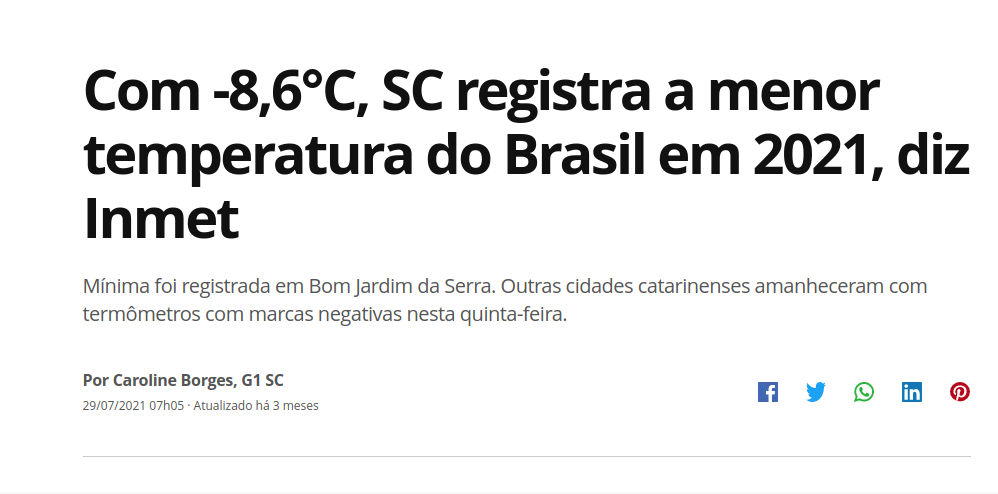
\includegraphics[scale = 0.3]{temp1.png}
    \caption{Registro da menor temperatura do Brasil- Fonte: G1}
    \label{fig:my_label}
\end{figure}
No Brasil, a unidade de medida usada oficialmente para a temperatura é o \textbf{grau Celsius}. Quando precisamos registrar medidas de temperaturas abaixo de \textbf{zero graus Célsius}, fazemos uso dos números negativos. Observe abaixo um exemplo de um \textbf{termômetro} com uma escala capaz de medir temperaturas abaixo de zero graus Celsius.
\begin{figure}[htb]
    \centering
    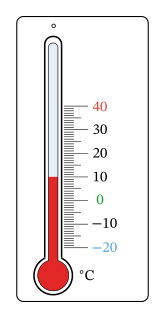
\includegraphics[scale=0.6]{term.png}
    \caption{Termômetro que registra temperaturas abaixo de zero}
    \label{fig:my_label}
\end{figure}
\section{Altitude}
Os números positivos e negativos também são utilizados para representar as altitudes. Consideramos o nível do mar igual a zero. Toda altitude que se encontra acima do nível do mar é representada por um valor positivo e toda altitude que fica abaixo do nível do mar é representada por um valor negativo. 
Para se ter uma ideia, o ponto mais alto da superfície da Terra em relação ao nível do mar fica no topo do monte Everest, no Nepal. O pico do Everest fica a 8.850 metros acima do nível do mar. O ponto de menor altitude (ou de maior profundidade) encontra-se na fossa das Marianas a 11.500 metros abaixo do mar. 
\begin{figure}[htb]
    \centering
    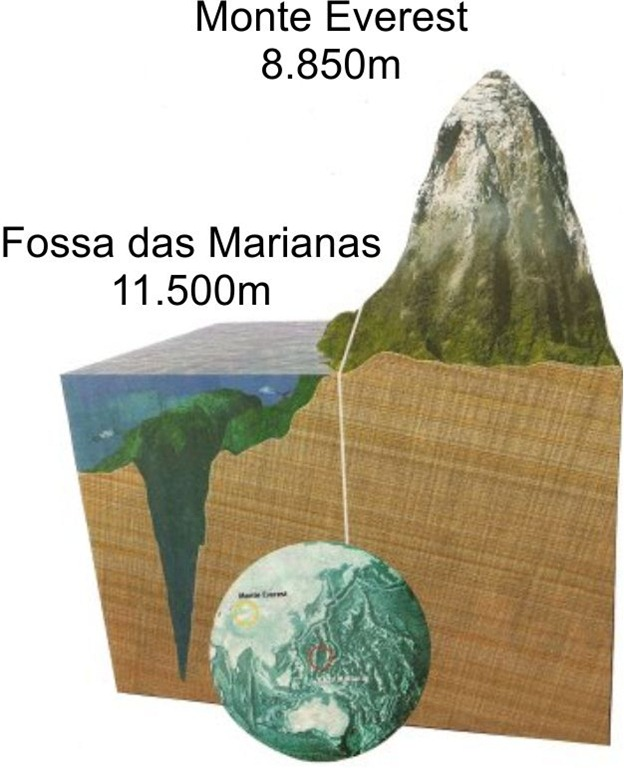
\includegraphics[scale =0.5]{fossa-das-marianas-2.jpg}
    \caption{Altitude da fossa das Marianas e do monte Everest}
    \label{fig:my_label}
\end{figure}
\section{Fuso horário civil}
Os fusos horários são divisões feitas sobre o planeta Terra. Ao todo, são 24 pedaços. Cada fuso horário mede 15º de longitude. Assim, cada fuso horário corresponde a 1 hora.Os fusos horários são medidos a partir do Meridiano de Greenwich. 
\\
À medida que nos distanciamos do meridiano de Greenwich para a esquerda do mapa, o horário vai se atrasando. Por outro lado, à medida que avançamos para a direita do meridiano de Greenwich, a hora fica adiantada em relação ao meridiano zero. 
\begin{figure}[htb]
    \centering
    \includegraphics[scale = 0.3]{5-1.png}
    \caption{Fusos horários}
    \label{fig:my_label}
\end{figure}
Podemos usar os números positivo e negativos para representar, respectivamente, os horários adiantados e atrasados em relação a Greenwich. 
\begin{itemize}
    \item Fuso horário positivo - Adiantado em relação a Greenwich.
    \item Fuso horário zero - Horário de Greenwich.
    \item Fuso horário negativo - Atrasado em relação ao horário de Greenwich.
\end{itemize}
\section{Valor monetário}
Os números negativos são muito utilizados em operações financeiras. Por exemplo, quando precisamos indicar um saldo negativo em uma conta bancária ou quando queremos indicar um prejuízo. Ou seja: 
\begin{itemize}
    \item Números positivos: se referem a um saldo bancário positivo. 
    \item Números negativos: se referem um saldo devedor.  
\end{itemize}
\end{document}